\documentclass{beamer}
\usepackage{tikz,amsmath,amssymb,hyperref,graphicx,stackrel,animate}
\usetikzlibrary{positioning,shadows,arrows,shapes,calc}
\newcommand{\argmax}{\operatornamewithlimits{argmax}}
\newcommand{\argmin}{\operatornamewithlimits{argmin}}
\mode<presentation>{\usetheme{Frankfurt}}
\AtBeginSection[]
{
  \begin{frame}<beamer>
    \frametitle{Outline}
    \tableofcontents[currentsection,currentsubsection]
  \end{frame}
}
\title{Lecture 18: Power Spectrum}
\author{Mark Hasegawa-Johnson\\All content~\href{https://creativecommons.org/licenses/by-sa/4.0/}{CC-SA 4.0} unless otherwise specified.}
\date{ECE 401: Signal and Image Analysis, Fall 2020}  
\begin{document}

% Title
\begin{frame}
  \maketitle
\end{frame}

% Title
\begin{frame}
  \tableofcontents
\end{frame}

%%%%%%%%%%%%%%%%%%%%%%%%%%%%%%%%%%%%%%%%%%%%
\section[Motivation]{Motivation: Noisy Telephones}
\setcounter{subsection}{1}

\begin{frame}
  \frametitle{Noisy Telephones}
  \begin{itemize}
  \item In the 1920s, Harvey Fletcher had a problem.
  \item Telephones were noisy (very noisy).
  \item Sometimes, people could hear the speech.  Sometimes not.
  \item Fletcher needed to figure out why people could or couldn't hear the
    speech, and what Western Electric could do about  it.
  \end{itemize}
\end{frame}

\begin{frame}
  \frametitle{Tone-in-Noise Masking Experiments}

  He began playing people pure tones mixed with noise, and asking
  people ``do you hear a tone''?  If 50\% of samples actually
  contained a tone, and if the listener was right 75\% of the time, he
  considered the tone ``audible.''
  \centerline{\includegraphics[height=2in]{exp/tone_white_waveform.png}}
\end{frame}

\begin{frame}
  \frametitle{Tone-in-Noise Masking Experiments}

  People's ears are astoundingly good.  This tone is inaudible in this
  noise.  But if the tone was only $2\times$ greater amplitude, it
  would be audible.
  \centerline{\includegraphics[height=2in]{exp/tone_white_waveform.png}}
\end{frame}

\begin{frame}
  \frametitle{Tone-in-Noise Masking Experiments}

  Even more astounding: the same tone, in a very slightly different noise,
  is perfectly audible, to every listener.
  \centerline{\includegraphics[height=2in]{exp/tone_bandstop_waveform.png}}
\end{frame}

\begin{frame}
  \frametitle{What's going on (why can listeners hear the tone?)}
  \centerline{\includegraphics[height=1.5in]{exp/tone_white_waveform.png}}
  \centerline{\includegraphics[height=1.5in]{exp/tone_bandstop_waveform.png}}
\end{frame}

%%%%%%%%%%%%%%%%%%%%%%%%%%%%%%%%%%%%%%%%%%%%
\section[Filters]{Auditory Filters}
\setcounter{subsection}{1}

\begin{frame}
  \frametitle{Review: Discrete Time Fourier Transform}

  Remember the discrete time Fourier transform (DTFT):
  \[
  X(\omega) = \sum_{n=-\infty}^{\infty} x[n]e^{-j\omega n},~~~
  x[n]=\frac{1}{2\pi}\int_{-\pi}^\pi |X(\omega)|e^{j\omega n}d\omega
  \]
  If the signal is only $N$ samples in the time domain, we can
  calculate samples of the DTFT using a  discrete Fourier transform:
  \[
  X[k] = X\left(\omega_k=\frac{2\pi k}{N}\right)=\sum_{n=0}^\infty x[n]e^{-j\frac{2\pi kn}{N}}
  \]
  We sometimes write this as $X[k]=X(\omega_k)$, where, obviously, $\omega_k=\frac{2\pi k}{N}$.
\end{frame}
  
\begin{frame}
  \frametitle{What's going on (why can listeners hear the tone?)}
  \centerline{\includegraphics[height=1.5in]{exp/tone_white_waveform.png}}
  \centerline{\includegraphics[height=1.5in]{exp/tone_bandstop_waveform.png}}
\end{frame}

\begin{frame}
  \frametitle{Fourier to the Rescue}

  Here's the DFT power spectrum ($|X[k]|^2$) of the tone, the white
  noise, and the combination.
  \centerline{\includegraphics[height=2in]{exp/tone_white_powerspectrum.png}}
\end{frame}

\begin{frame}
  \frametitle{Bandstop Noise}

  The ``bandstop'' noise is called ``bandstop'' because I arbitrarily set
  its power to zero in a small frequency band centered at 1kHz.  Here is the
  power spectrum.  Notice that, when the tone is added to the noise signal, 
  the little bit of extra power makes a noticeable (audible) change, because
  there is no other power at that particular frequency.
  \centerline{\includegraphics[height=2in]{exp/tone_bandstop_powerspectrum.png}}
\end{frame}

\begin{frame}
  \frametitle{Fletcher's Model of Masking}

  Fletcher proposed the following model of hearing in noise:
  \begin{enumerate}
  \item The human ear pre-processes  the audio using a bank of bandpass filters.
  \item The power of the noise signal, in the $k^{\textrm{th}}$
    bandpass filter, is $N_k$.
  \item The power of the noise+tone is $N_k+T_k$.
  \item If there is {\bf\em any} band, $k$, in which
    $\frac{N_k+T_k}{N_k}>\mbox{threshold}$, then the tone is audible.
    Otherwise, not.
  \end{enumerate}
\end{frame}

\begin{frame}
  \frametitle{Von Bekesy and the Basilar Membrane}

  \begin{itemize}
  \item In 1928, Georg von B{\'{e}}k{\'{e}}sy found Fletcher's auditory
    filters.
  \item Surprise: they are {\bf\em mechanical}.
  \item The inner ear contains a long (3cm), thin (1mm), tightly
    stretched membrane (the basilar membrane).  Like a steel drum, it
    is tuned to different frequencies at different places: the outer
    end is tuned to high frequencies, the inner end to low
    frequencies.
  \item About 30,000 nerve cells lead from the basilar membrane to the
    brain stem.  Each one sends a signal if its part of the basilar
    membrane vibrates.
  \end{itemize}
\end{frame}

\begin{frame}
  \centerline{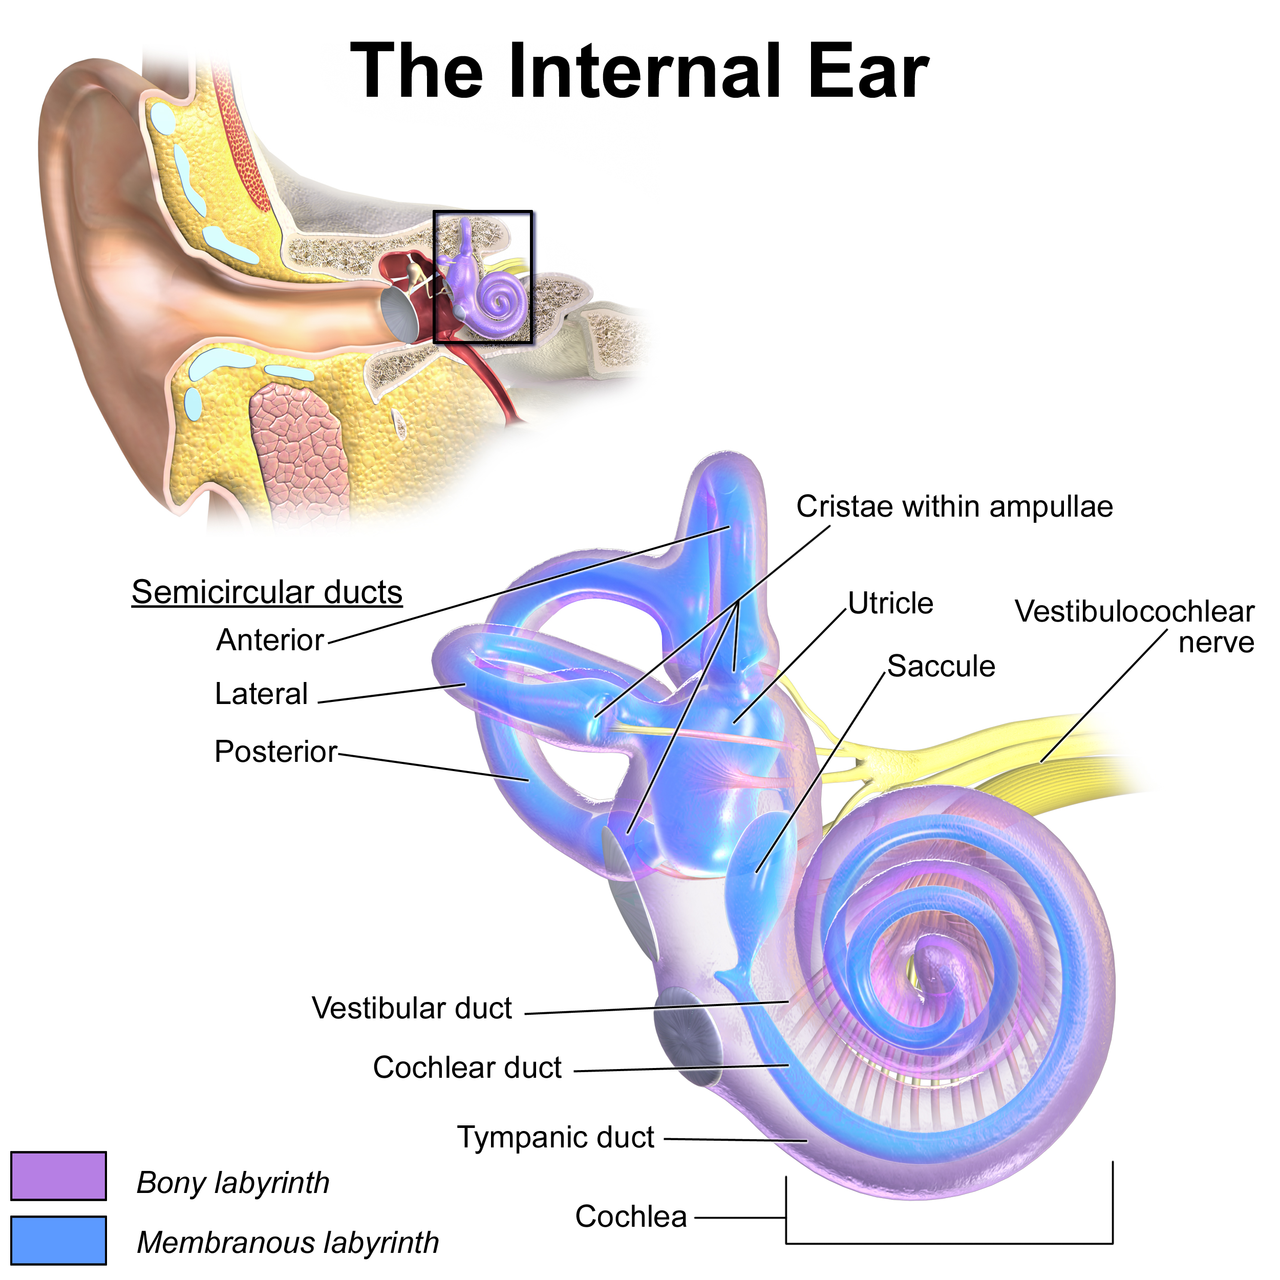
\includegraphics[height=3in]{Blausen_0329_EarAnatomy_InternalEar.png}}
  \begin{tiny}
    Blausen.com staff (2014). ``Medical gallery of Blausen Medical
    2014.'' WikiJournal of Medicine 1
    (2). DOI:10.15347/wjm/2014.010. ISSN 2002-4436.
  \end{tiny}
\end{frame}

\begin{frame}
  \centerline{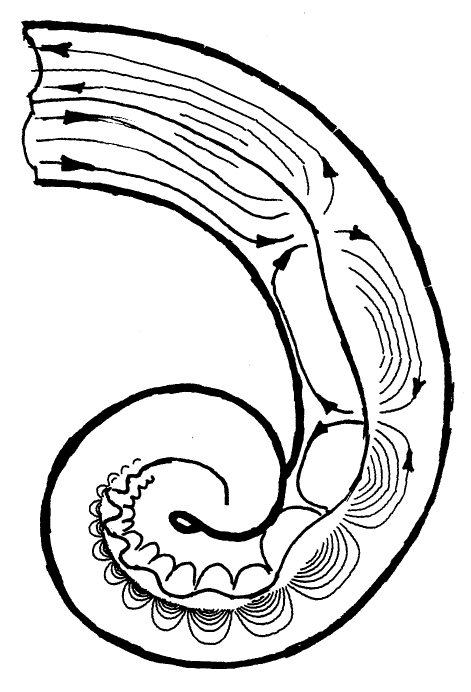
\includegraphics[height=3in]{Cochlea_Traveling_Wave.png}}
  \begin{tiny}
    Dick Lyon, public domain image, 2007.
    \url{https://en.wikipedia.org/wiki/File:Cochlea_Traveling_Wave.png}
  \end{tiny}
\end{frame}

\begin{frame}
  \frametitle{Frequency responses of the auditory filters}

  Here are the squared magnitude frequency responses ($|H(\omega)|^2$)
  of 26 of the 30000 auditory filters. I plotted these using the
  parametric model published by Patterson in 1974:
  \centerline{\includegraphics[height=2in]{exp/gammatone_filterbank.png}}
\end{frame}
     
\begin{frame}
  \frametitle{Filtered white noise}

  An acoustic white  noise signal (top), filtered through a spot on the
  basilar membrane with a particular impulse response (middle), might result in
  narrowband-noise  vibration of the basilar membrane (bottom).
  \centerline{\includegraphics[height=2in]{exp/gtfiltered_white_waveform.png}}
\end{frame}
     
\begin{frame}
  \frametitle{Filtered white noise}

  An acoustic white  noise signal (top), filtered through a spot on the
  basilar membrane with a particular impulse response (middle), might result in
  narrowband-noise  vibration of the basilar membrane (bottom).
  \centerline{\includegraphics[height=2in]{exp/gtfiltered_white_powerspectrum.png}}
\end{frame}
     
\begin{frame}
  \frametitle{Tone + Noise: Waveform}

  If there is a tone embedded in the noise, then even after filtering, it's
  very hard to see that the tone is there\ldots
  
  \centerline{\includegraphics[height=2in]{exp/gtfiltered_tone_white_waveform.png}}
\end{frame}
     
\begin{frame}
  \frametitle{Filtered white noise}

  But, Fourier comes to the rescue!  In the power spectrum, it is
  almost possible, now, to see that the tone is present in the white noise masker.
  
  \centerline{\includegraphics[height=2in]{exp/gtfiltered_tone_white_powerspectrum.png}}
\end{frame}
     
\begin{frame}
  \frametitle{Filtered bandstop noise}

  If the masker is bandstop noise, instead of white noise, the spectrum
  after filtering looks very different\ldots
  
  \centerline{\includegraphics[height=2in]{exp/gtfiltered_bandstop_powerspectrum.png}}
\end{frame}
     
\begin{frame}
  \frametitle{Filtered tone + bandstop noise}

  \ldots and the tone+noise looks very, very different from the noise by itself.
  \centerline{\includegraphics[height=2in]{exp/gtfiltered_tone_bandstop_powerspectrum.png}}
  \centerline{\huge This is why the tone is audible!}
\end{frame}

\begin{frame}
  \frametitle{What an excellent model!  Why should  I believe it?}

  Now that  you've seen the pictures, it's time to learn the math.
  \begin{itemize}
  \item What is white noise?
  \item What is a power spectrum?
  \item What is filtered noise?
  \end{itemize}
  Let's find out.
\end{frame}

%%%%%%%%%%%%%%%%%%%%%%%%%%%%%%%%%%%%%%%%%%%%
\section[White Noise]{White Noise}
\setcounter{subsection}{1}

\begin{frame}
  \frametitle{What is Noise?}

  By ``noise,'' we mean a signal $x[n]$ that is unpredictable.  In
  other words, each sample of $x[n]$ is a random variable.
\end{frame}

\begin{frame}
  \frametitle{What is White Noise?}

  ``White noise'' is a noise signal where each sample, $x[n]$, is
  {\bf uncorrelated} with all the other samples.   Using $E[\cdot]$
  to mean ``expected value,'' we can write:
  \begin{align*}
    E\left[x[n]x[n+m]\right] &= E\left[x[n]\right]E\left[x[n+m]\right]~~\mbox{for}~m\ne 0
  \end{align*}
      {\bf Most noises are not white noise.}  The equation above is
      only true for white noise.  White noise is really useful, so
      we'll work with this equation a lot, but it's important to
      remember:
      {\bf Only white noise has uncorrelated samples}.
\end{frame}

\begin{frame}
  \frametitle{What is Zero-Mean, Unit-Variance White Noise?}

  Zero-mean, unit-variance white noise is noise with uncorrelated samples,
  each of which has zero mean:
  \begin{align*}
    \mu = E\left[x[n]\right] & = 0
  \end{align*}
  and unit variance:
  \begin{align*}
    \sigma^2 = E\left[\left(x[n]-\mu\right)^2\right] &= 1
  \end{align*}
  Putting the above together with the definition of white noise, we get
  \begin{align*}
    E\left[x[n]x[n+m]\right] &= \begin{cases}
      1 & m=0\\ 0 &m\ne 0\end{cases}
  \end{align*}
\end{frame}

\begin{frame}
  \frametitle{What is the Spectrum of White Noise?}

  Let's try taking the Fourier transform of zero-mean, unit-variance white noise:
  \begin{displaymath}
    X(\omega) = \sum_{n=-\infty}^{\infty} x[n]e^{-j\omega n}
  \end{displaymath}
  The right-hand side of the equation is random, so {\bf the left-hand
    side is random too}.  In other words, if $x[n]$ is noise, then
  \begin{itemize}
  \item for any particular frequency, $\omega$, that you want to investigate,
  \item $X(\omega)$ is a random variable.
  \item It has a random real part  ($X_R(\omega)$)
  \item It has a random imaginary part  ($X_I(\omega)$).
  \end{itemize}
\end{frame}

\begin{frame}
  \frametitle{What is the Average Fourier Transform of White Noise?}

  Since $X(\omega)$ is a random variable, let's find its expected value.
  \begin{align*}
    E\left[X(\omega)\right] &= E\left[\sum_{n=-\infty}^{\infty} x[n]e^{-j\omega n}\right]
  \end{align*}
  Expectation is linear, so we can write
  \begin{align*}
    E\left[X(\omega)\right] &= \sum_{n=-\infty}^{\infty} E\left[x[n]\right] e^{-j\omega n}
  \end{align*}
  But $E\left[x[n]\right]=0$!  So
  \begin{align*}
    E\left[X(\omega)\right] &= 0
  \end{align*}
  That's kind of disappointing, really.  Who knew noise could be so boring?
\end{frame}

\begin{frame}
  \frametitle{What is the Average Squared Magnitude Spectrum of White Noise?}

  Fortunately, the squared magnitude spectrum, $|X(\omega)|^2$, is a little more interesting:
  \begin{align*}
    E\left[|X(\omega)|^2\right] &=  E\left[X(\omega)X^*(\omega)\right]
  \end{align*}
  Goodness.  What is that?  Let's start out by trying to figure out what is  $X^*(\omega)$, the
  complex conjugate of $X(\omega)$.
\end{frame}

\begin{frame}
  \frametitle{What is the Complex Conjugate of a Fourier Transform?}

  First, let's try to figure out what $X^*(\omega)$ is:
  \begin{align*}
    X^*(\omega) &= \left({\mathcal F}\left\{x[m]\right\}\right)^*\\
    &= \left(\sum_{m=-\infty}^\infty x[m]e^{-j\omega m}\right)^*\\
    &= \sum_{m=-\infty}^\infty x[m]e^{j\omega m}\\
  \end{align*}
\end{frame}

\begin{frame}
  \frametitle{Average Squared Magnitude Spectrum?}

  Now let's plug back in here:
  \begin{align*}
    E\left[|X(\omega)|^2\right] &=  E\left[X(\omega)X^*(\omega)\right]\\
    &= E\left[\left(\sum_{n=-\infty}^\infty x[n]e^{-j\omega n}\right)
      \left(\sum_{m=-\infty}^\infty x[m]e^{j\omega m}\right)\right]\\
    &= E\left[\sum_{n=-\infty}^\infty\sum_{m=-\infty}^\infty x[n]x[m]e^{j\omega(m-n)}\right]\\
    &= \sum_{n=-\infty}^\infty\sum_{m=-\infty}^\infty E\left[x[n]x[m]\right]e^{j\omega(m-n)}
  \end{align*}
  But remember the definition of zero-mean white noise: $E\left[x[n]x[m]\right]=0$ unless $n=m$.
  So
  \begin{align*}
    E\left[|X(\omega)|^2\right] &=  \sum_{n=-\infty}^\infty E\left[x^2[n]\right]
  \end{align*}
\end{frame}

\begin{frame}
  \frametitle{Energy Spectrum is Infinity!!  Oops.}

  We have proven that the expected squared-magnitude Fourier transform
  of zero-mean, unit-variance white noise is a constant:
  \begin{align*}
    E\left[|X(\omega)|^2\right] &=  \sum_{n=-\infty}^\infty E\left[x^2[n]\right]
    &=  \sum_{n=-\infty}^\infty 1
  \end{align*}
  Unfortunately, the constant is infinity!
\end{frame}
\begin{frame}
  \frametitle{Power Spectrum}
  
  Wiener solved this problem
  by defining something called the {\bf Power Spectrum:}
  \begin{align*}
    R_{xx}(\omega)  &= \lim_{N\rightarrow\infty} \frac{1}{N}\left|\sum_{n=-(N-1)/2}^{(N-1)/2} x[n]e^{-j\omega n}\right|^2
  \end{align*}
\end{frame}

\begin{frame}
  \frametitle{What is power?}

  \begin{itemize}
    \item Power (Watts=Joules/second) is energy (in Watts) per unit time (in seconds).
    \item Example: electrical energy = volts$\times$charge,
      power=volts$\times$current (current = charge/time)
    \item Example: mechanical energy = force$\times$distance,
      power=force$\times$velocity (velocity = distance/time)
  \end{itemize}
\end{frame}

\begin{frame}
  \frametitle{Power Spectrum of White Noise}

  So the power spectrum of white noise is
  \begin{displaymath}
    R_{xx}(\omega) = \lim_{N\rightarrow\infty} \frac{1}{N} |X(\omega)|^2
  \end{displaymath}
  where $N$ is the number of samples over which we computed the Fourier transform.
\end{frame}
\begin{frame}
  \frametitle{Power Spectrum of White Noise}
  And now here's why white noise is called ``white:''
  \begin{align*}
    E\left[R_{xx}(\omega)\right] &= \frac{1}{N}E\left[|X(\omega)|^2\right]\\
    &=  \frac{1}{N}\sum_{n=-(N-1)/2}^{(N-1)/2} E\left[x^2[n]\right]\\
    &=  \frac{1}{N}\sum_{n=-(N-1)/2}^{(N-1)/2} 1\\
    &= 1
  \end{align*}
  The power spectrum of white noise is, itself, a random variable; but
  its expected value is the power of $x[n]$,
  \begin{displaymath}
    E\left[R_{xx}(\omega)\right] = E[x^2[n]]=1
  \end{displaymath}
\end{frame}

%%%%%%%%%%%%%%%%%%%%%%%%%%%%%%%%%%%%%%%%%%%%
\section[Colors]{Noise of Many Colors}
\setcounter{subsection}{1}

\begin{frame}
  \frametitle{The Power Spectrum of Filtered Noise}

  Suppose that we filter the white noise, like this:
  \begin{displaymath}
    y[n]=h[n]\ast x[n]~~~\leftrightarrow~~~Y(\omega) =H(\omega)X(\omega)
  \end{displaymath}
\end{frame}

\begin{frame}
  \frametitle{Power Spectrum of Filtered Noise}

  The power spectrum of the filtered noise will be
  \begin{align*}
    R_{yy}(\omega) &= \lim_{N\rightarrow\infty} \frac{1}{N} |H(\omega)X(\omega)|^2\\
    &= |H(\omega)|^2 R_{xx}(\omega)\\
    &= |H(\omega)|^2
  \end{align*}
  where $N$ is the number of samples over which we computed the Fourier transform.
\end{frame}

\begin{frame}
  \frametitle{Colors, anybody?}

  \begin{itemize}
    \item Noise with a flat power spectrum (uncorrelated samples) is
      called white noise.
    \item Noise that has been filtered (correlated samples) is called
      colored noise.
      \begin{itemize}
      \item If it's a low-pass filter, we call it pink noise (this is
        quite standard).
      \item If it's a high-pass filter, we could call it blue noise
        (not so standard).
      \item If it's a band-pass filter, we could call it green noise
        (not at all standard, but I like it!)
      \end{itemize}
  \end{itemize}
\end{frame}

\begin{frame}
  \frametitle{What is the Power of Filtered Noise?}

  Remember that, for white noise, we had
  \begin{displaymath}
    E\left[R_{xx}(\omega)\right] = E[x^2[n]]=1
  \end{displaymath}
  The same thing turns out to be true for filtered noise:
  \begin{align*}
    E\left[y^2[n]\right] &= \mbox{average}\left(E\left[R_{yy}(\omega)\right]\right)\\
    &= \frac{1}{2\pi}\int_{-\pi}^\pi E\left[R_{yy}(\omega)\right]d\omega
  \end{align*}
\end{frame}

\begin{frame}
  \frametitle{Power of White Noise: Example}

  For example, here is a white noise signal $x[n]$, and its power
  spectrum $R_{xx}(\omega)=\frac{1}{N}|X(\omega)|^2$:
  \centerline{\includegraphics[height=2in]{exp/whitefreqandtime.png}}
\end{frame}

\begin{frame}
  \frametitle{Power of Pink Noise: Example}

  Here's the same signal, after filtering with a lowpass filter with cutoff $\pi/2$:
  \centerline{\includegraphics[height=2in]{exp/pinkfreqandtime.png}}
\end{frame}

\begin{frame}
  \frametitle{Power of Blue Noise: Example}

  Here's the same signal, after filtering with a highpass filter with cutoff $\pi/2$:
  \centerline{\includegraphics[height=2in]{exp/bluefreqandtime.png}}
\end{frame}

\begin{frame}
  \frametitle{Parseval's Theorem}

  The relationship between energy in the time domain and energy in the
  frequency domain is summarized by Parseval's theorem.  There is a
  form of Parseval's theorem for every type of Fourier transform.  For
  the DTFT, it is
  \begin{displaymath}
    \sum_{n=-\infty}^\infty x^2[n] = \frac{1}{2\pi}\int_{-\pi}^\pi |X(\omega)|^2d\omega
  \end{displaymath}
  For the DFT, it is:
  \begin{displaymath}
    \sum_{n=0}^{N-1} x^2[n] = \frac{1}{N}\sum_{k=0}^{N-1}|X[k]|^2
  \end{displaymath}
\end{frame}

\begin{frame}
  \frametitle{Parseval's Theorem}

  For the power spectrum, Parseval's theorem says that power is the same in
  both time domain and frequency domain:
  \begin{displaymath}
    \lim_{N\rightarrow\infty}\frac{1}{N}\sum_{n=-(N-1)/2}^{(N-1)/2)} x^2[n] =
    \frac{1}{2\pi}\int_{-\pi}^\pi R_{xx}(\omega)\omega
  \end{displaymath}
  The DFT version of power is:
  \begin{displaymath}
    \frac{1}{N}\sum_{n=0}^{N-1} x^2[n] = \frac{1}{N}\sum_{k=0}^{N-1}|R_{xx}(\omega_k)|^2
  \end{displaymath}
\end{frame}





%%%%%%%%%%%%%%%%%%%%%%%%%%%%%%%%%%%%%%%%%%%%
\section[Summary]{Summary}
\setcounter{subsection}{1}

\begin{frame}
  \frametitle{Summary}
  \begin{itemize}
  \item Masking: a pure tone can be heard, in noise, if there is {\bf at least one}
    auditory filter through which $\frac{N_k+T_k}{N_k}>$ threshold.
  \item Zero-mean, unit-variance white Noise: samples of $x[n]$ are
    uncorrelated, so the expected power spectrum is:
    \begin{displaymath}
      E\left[R_{xx}(\omega)\right] = 1
    \end{displaymath}
  \item Power spectrum in general: The relationship between power in
    the time domain, and power in the frequency domain, in general, is
    given by {\bf Parseval's Theorem:}
    \begin{displaymath}
      \sum_{n=-\infty}^\infty x^2[n] = \frac{1}{2\pi}\int_{-\pi}^\pi |X(\omega)|^2d\omega
    \end{displaymath}
    \begin{displaymath}
      \lim_{N\rightarrow\infty}\frac{1}{N}\sum_{n=-(N-1)/2}^{(N-1)/2)} x^2[n] =
      \frac{1}{2\pi}\int_{-\pi}^\pi R_{xx}(\omega)\omega
    \end{displaymath}
  \end{itemize}
\end{frame}

\end{document}
